\documentclass[12pt,border=2pt]{standalone}
\usepackage[T1]{fontenc}
\usepackage{amsmath}
\usepackage{mathpazo}
\usepackage{tikz}
\usetikzlibrary{arrows.meta}
\begin{document}
% Panel (a) of the Bezier figure in the KAN subsection of Section 2.1: a cubic Bezier curve,
% its control points V_1..V_4 and their convex hull (same points as slide 1 of the deck).
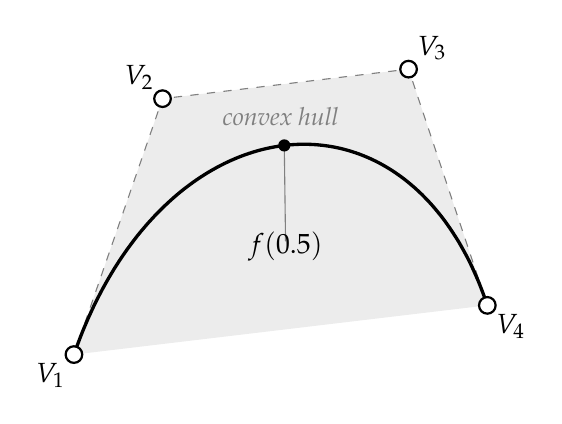
\begin{tikzpicture}[x=1.25cm, y=1.25cm]
  \fill[gray!15] (0.0,0.0) -- (0.9,2.6) -- (3.4,2.9) -- (4.2,0.5) -- cycle;
  \draw[gray, dashed] (0.0,0.0) -- (0.9,2.6) -- (3.4,2.9) -- (4.2,0.5);
  \draw[very thick] plot coordinates {(0.000,0.0000) (0.023,0.0651) (0.047,0.1291) (0.071,0.1922) (0.096,0.2544) (0.122,0.3155) (0.148,0.3757) (0.175,0.4349) (0.202,0.4931) (0.230,0.5503) (0.259,0.6065) (0.288,0.6617) (0.318,0.7160) (0.348,0.7692) (0.379,0.8215) (0.410,0.8728) (0.442,0.9230) (0.474,0.9723) (0.507,1.0206) (0.540,1.0679) (0.574,1.1141) (0.608,1.1594) (0.642,1.2037) (0.677,1.2469) (0.713,1.2892) (0.748,1.3304) (0.785,1.3706) (0.821,1.4099) (0.858,1.4481) (0.895,1.4853) (0.933,1.5214) (0.971,1.5566) (1.009,1.5908) (1.047,1.6239) (1.086,1.6560) (1.125,1.6871) (1.165,1.7171) (1.204,1.7461) (1.244,1.7741) (1.284,1.8011) (1.325,1.8271) (1.365,1.8520) (1.406,1.8758) (1.447,1.8987) (1.488,1.9205) (1.529,1.9413) (1.570,1.9610) (1.612,1.9797) (1.653,1.9973) (1.695,2.0139) (1.737,2.0295) (1.779,2.0440) (1.821,2.0575) (1.863,2.0699) (1.905,2.0813) (1.947,2.0916) (1.990,2.1009) (2.032,2.1091) (2.074,2.1162) (2.116,2.1223) (2.159,2.1274) (2.201,2.1314) (2.243,2.1343) (2.285,2.1361) (2.327,2.1369) (2.369,2.1367) (2.411,2.1353) (2.453,2.1329) (2.494,2.1294) (2.536,2.1249) (2.577,2.1193) (2.619,2.1126) (2.660,2.1048) (2.701,2.0960) (2.742,2.0860) (2.782,2.0750) (2.823,2.0629) (2.863,2.0498) (2.903,2.0355) (2.942,2.0202) (2.982,2.0037) (3.021,1.9862) (3.060,1.9676) (3.099,1.9479) (3.137,1.9271) (3.175,1.9052) (3.213,1.8823) (3.250,1.8582) (3.287,1.8330) (3.324,1.8067) (3.360,1.7794) (3.396,1.7509) (3.431,1.7213) (3.467,1.6906) (3.501,1.6588) (3.536,1.6259) (3.569,1.5919) (3.603,1.5568) (3.636,1.5205) (3.668,1.4832) (3.700,1.4447) (3.732,1.4051) (3.763,1.3644) (3.793,1.3226) (3.823,1.2797) (3.852,1.2356) (3.881,1.1904) (3.910,1.1441) (3.937,1.0967) (3.964,1.0481) (3.991,0.9984) (4.017,0.9475) (4.042,0.8956) (4.066,0.8425) (4.090,0.7883) (4.114,0.7329) (4.136,0.6764) (4.158,0.6187) (4.179,0.5599) (4.200,0.5000)};
  \draw[gray] (2.137,2.125) -- (2.15,1.15);
  \fill (2.137,2.125) circle (2.2pt);
  \node[anchor=north] at (2.15,1.35) {$f(0.5)$};
  \node[font=\small\itshape, gray] at (2.1,2.42) {convex hull};
  \draw[thick, fill=white] (0.0,0.0) circle (3pt);
  \node[anchor=north east, inner sep=3pt] at (0.0,0.0) {$V_1$};
  \draw[thick, fill=white] (0.9,2.6) circle (3pt);
  \node[anchor=south east, inner sep=3pt] at (0.9,2.6) {$V_2$};
  \draw[thick, fill=white] (3.4,2.9) circle (3pt);
  \node[anchor=south west, inner sep=3pt] at (3.4,2.9) {$V_3$};
  \draw[thick, fill=white] (4.2,0.5) circle (3pt);
  \node[anchor=north west, inner sep=3pt] at (4.2,0.5) {$V_4$};
\end{tikzpicture}
\end{document}
